\chapter{Quy trình phát triển phần mềm nhúng}

%================ Requirement ===================
    \section{Xác định yêu cầu người dùng}
        Việc phát triển một hệ thống nhúng thường có nhiều người yêu cầu, bao
        gồm: nhà sản xuất phần cứng, người bảo trì, marketing, khách hàng (hình
        \ref{fig:stakeholder})\cite{EmbSysState}.

        \begin{figure}[H]
            \centering
            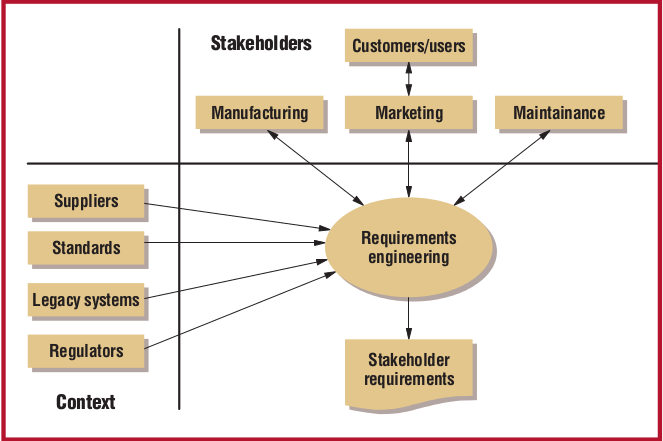
\includegraphics[scale=0.6]{stakeholder}
            \rule{35em}{0.5pt}
            \caption{Các bên yêu cầu (stakeholder) trong một dự án hệ thống nhúng}
            \label{fig:stakeholder}
        \end{figure}

        Bước đầu, khách hàng xác định các yêu cầu chức năng
        (\texttt{functional}) và các yêu cầu phi chức năng
        (\texttt{non-functional}). Tuỳ thuộc vào loại sản phẩm mà khách hàng sẽ
        đàm phán qua bộ phận marketing hay trực tiếp với các nhà phát triển.

        Kết quả của bước này sẽ là một bản đặc tả các yêu cầu, mô tả về hệ
        thống sao cho tất cả các bên yêu cầu đều có thể hiểu được. Tài liệu này
        được coi như hợp đồng với nhà phát triển (phần mềm nhúng).

        \paragraph{Đặc tả yêu cầu}

        Với phần mềm nhúng, các đặc tả phi chức năng (\texttt{non-functional
        specification}) rất quan trọng (do các ràng buộc về tài nguyên hạn chế,
        đáp ứng ở thời gian thực, mức tiêu thụ năng lượng, \ldots). Mà đặc tả
        phi chức năng thường rất khó phát biểu chính xác, do đó không
        thể dùng các phương pháp đặc tả yêu cầu như bình thường (như sử dụng
        các mẫu (template) của các trình soạn thảo văn bản).

        Với những dự án có sử dụng các biểu đồ để đặc tả, các biểu đồ này hầu
        hết ở dạng tự do hoặc các biểu đồ tương tự với UML, DFD
        (\texttt{Dataflow diagrams} - biểu đồ luồng dữ liệu), \ldots. Do không
        có một sự thống nhất về cú pháp của các biểu đồ, các thành viên dự án
        có thể hiểu sai ý nghĩa của nó.

        Đặc tả hình thức (\texttt{formal specification}) thường ít được sử
        dụng do tính phức tạp của hệ thống nhúng cũng như các yêu cầu của nó.
        Việc sử dụng đặc tả hình thức sẽ làm sự hợp tác giữa các thành viên
        trong dự án trở nên khó khăn hơn vì hầu hết các thành viên đều không
        hoàn toàn hiểu nó. Với khách hàng thì vấn đề này còn khó khăn hơn nữa.

%=============== Thiết kế ========================
    \section{Thiết kế}
        \subsection{Thiết kế hệ thống}
            Các hệ thống nhúng 

        \subsection{Thiết kế chương trình}
            \paragraph{Thiết kế hướng đối tượng / hướng thủ tục}
                Các phương pháp thiết kế này sử dụng các \texttt{thủ tục} (đối với
                thiết kế hướng đối tượng là \texttt{phương thức}) là các thành
                phần cơ bản của chương trình. Các thủ tục (phương thức) này
                nhận các tham số, thực hiện một số hữu hạn các phép tính và trả
                về giá trị.

                Phương pháp hướng đối tượng hợp nhất các thủ tục và dữ liệu để
                tạo thành các \texttt{đối tượng (object)}. Các đối tượng này là
                thụ động, bởi vì nó cần sự tác động của bên ngoài để thực hiện
                các phương thức của nó.

                Tuy nhiên thế giới thực là chủ động, giống với các tiến trình
                hơn là các đối tượng, nó hoạt động trên các luồng riêng, tương
                tác với các tiến trình khác bằng các thông điệp. 

                Như vậy, mặc dù thiết kế hướng đối tượng được sử dụng rất nhiều
                trong việc xây dựng các hệ thống phần mèm lớn, nó lại không
                thích hợp cho việc giải quyết các vấn đề của việc thiết kế phần
                mềm nhúng.

            \paragraph{Mô hình hướng đối tượng thời gian thực}
                Với những yêu cầu về thời gian thực của phần mềm nhúng, cần có
                một mô hình khác để biểu diễn vấn đề. Ở đây là mô hình hướng
                đối tượng thời gian thực (Real-time Object Oriented Modeling -
                ROOM). ROOM định nghĩa các mô hình đối tượng có thể diễn tả
                quan hệ giữa các đối tượng, biểu đồ trạng thái (\texttt{state
                diagram}) chỉ rõ các hành động của đối tượng, và 

%============ Coding =============================
    \section{Mã hoá chương trình}
        \paragraph{Ngôn ngữ lập trình}
            Do thường gặp hạn chế về tài nguyên cũng như yêu cầu về hiệu năng,
            C và Assembly là hai ngôn ngữ thường được sử dụng trong lập trình
            phần mềm nhúng. Chương trình viết bằng 2 ngôn ngữ này thường nhỏ,
            nhanh và có khả năng thao tác trực tiếp với phần cứng. Trong đó
            Assembly thường được dùng cho những nơi cần yêu cầu cao về hiệu
            năng, kích thước chương trình hay là phụ thuộc phần cứng (VD:
            driver).

            Mặc dù ngôn ngữ C không trực tiếp hỗ trợ lập trình hướng đối tượng
            nhưng vẫn có thể sử dụng các kỹ thuật hướng đối tượng bằng các cấu
            trúc có sẵn của C:
            \begin{itemize}
                \item Sử dụng struct thay cho class,
                \item Sử dụng hàm với đối số đầu kiểu của struct thay
                    cho phương thức,
                \item Sử dụng con trỏ void để có được khả năng đa hình,
                \item \ldots
            \end{itemize}


            Ngoài ra, cũng có thể dùng C++ cho phát triển phần mềm nhúng. C++
            kế thừa được những ưu điểm của C (mềm dẻo, hiệu năng) cộng thểm
            nhiều tính năng khác làm cho việc lập trình đơn giản hơn (template,
            STL, \ldots). Tuy vậy cần chú ý đến kích thước chương trình khi sử
            dụng các tính năng này. Ngoài ra một số tính năng như exception
            cũng có thể không được hỗ trợ trên một số hệ thống.

        \paragraph{Một số vấn đề khi mã hoá chương trình phần mềm nhúng}
            \subparagraph{Sự phụ thuộc nền tảng}
                Một chương trình có thể chạy đúng với phần cứng này, HDH này
                nhưng chưa chắc đã chạy đúng trên phần cứng, HDH khác. Đó là do
                một số yếu tố trong chương trình khác nhau ở những nền tảng
                khác nhau. Ví dụ:
                \begin{itemize}
                    \item Kích thước kiểu dữ liệu nguyên (\texttt{int, long,
                        short}, các
                        kiểu con trỏ): ngôn ngữ C/C++ không quy định về kích
                        thước chính xác của các kiểu dữ liệu này. VD: HDH 32bit
                        thường quy định kích thước con trỏ là 32bit, HDH 64bit
                        thường quy định kích thước con trỏ là 64bit. Do vậy cần
                        chú ý khi sử dụng các kiểu dữ liệu này, không nên mặc
                        nhiên coi rằng một kiểu dữ liệu nào đó có một kích
                        thước xác định. Nếu muốn kiểu nguyên với kích thước cụ
                        thể thì sử dụng các kiểu có sẵn như \texttt{int32\_t,
                        uint16\_t, \ldots}.
                    \item Sự căn chỉnh byte (byte alignment) và thứ tự byte
                        (byte order): Với mỗi hệ thống khác nhau, yêu cầu về
                        byte alignment và byte order có thể khác nhau. VD: trên
                        MIPS, truy cập vào một biến nguyên 32bit có địa chỉ
                        không chia hết cho 4 sẽ sinh ra lỗi SIGBUS.
                    \item Tính toán số thực dấu phẩy động: nhiều vi xử lý hiện nay
                        không hỗ trợ tính toán trên dấu phẩy động. Khi đưa
                        chương trình lên nền tảng này cần cân nhắc việc cài đặt
                        tính năng này bằng phần mềm hoặc sử dụng một thuật toán
                        khác không sử dụng đến tính toán số thực dấu phẩy động.
                \end{itemize}
            \subparagraph{Hạn chế về tài nguyên}
                Đây luôn là vấn đề xuyên suốt cả quá trình phát triển phần mềm
                nhúng. Trong gian đoạn mã hoá chương trình này, cần tuân thủ
                chặt chẽ các nguyên tắc để sự dụng tiết kiệm tài nguyên nhất có
                thể mà vẫn đảm bảo được hiệu năng.

        \paragraph{Công cụ}
            \subparagraph{Trình biên dịch (compiler)}
                Trình biên dịch được sử dụng trong lập trình nhúng là cross
                compiler, tức là trình dịch chạy trên host nhưng lại sinh mà
                cho target. Với mỗi target khác nhau sẽ có một cross compiler
                riêng, thường do các nhà sản xuất vi xử lý cung cấp. Ngoài ra
                còn có những trình biên dịch có thể sinh mã cho nhiều target
                khác nhau, như GCC hỗ trợ hơn 20 loại vi xử lý \cite{GccWiki}.

            \subparagraph{Trình dịch hợp ngữ (Assembler)}
                Chạy trên host. Có nhiệm vụ dịch mã hợp ngữ được sinh ra bởi
                compiler thành mã máy.

            \subparagraph{Trình liên kết (Linker)}
                Liên kết các file mã máy (nhị phân) đã được biên dịch cùng với
                các thư viện cần thiết thành chương trình hoàn chỉnh. Cũng chạy
                trên host.

            \subparagraph{Chương trình giả lập (emulator)}
                Giả lập target trên host. Dùng để debug hoặc test chương trình
                mà không cần phải sử dụng phần cứng thật (target). Emulator
                thường sử dụng phương pháp thông dịch mã nhị phân của target thành mã
                nhị phân dành cho máy host để máy host có thể hiểu và thực thi
                được chương trình. Do đó chương trình chạy trên emulator thường
                chậm hơn so với máy thực.


                \begin{figure}[H]
                    \centering
                    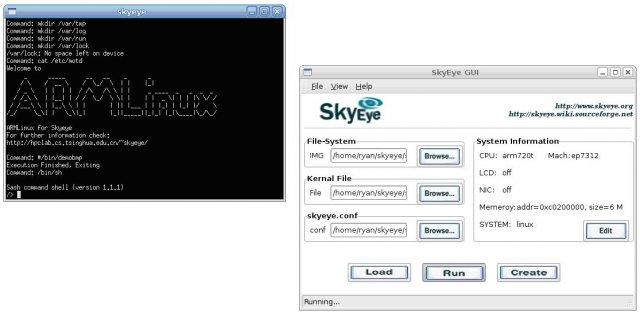
\includegraphics[scale=0.6]{armemu}
                    \rule{35em}{0.5pt}
                    \caption{Giả lập ARM trên PC x86}
                    \label{fig:armemu}
                \end{figure}

            \subsection{Môi trường phát triển tích hợp}
                Chương trình hợp nhất tất cả các công cụ phát triển (compiler, assembler,
                linker, emulator, \ldots).
                

                \begin{figure}[H]
                    \centering
                    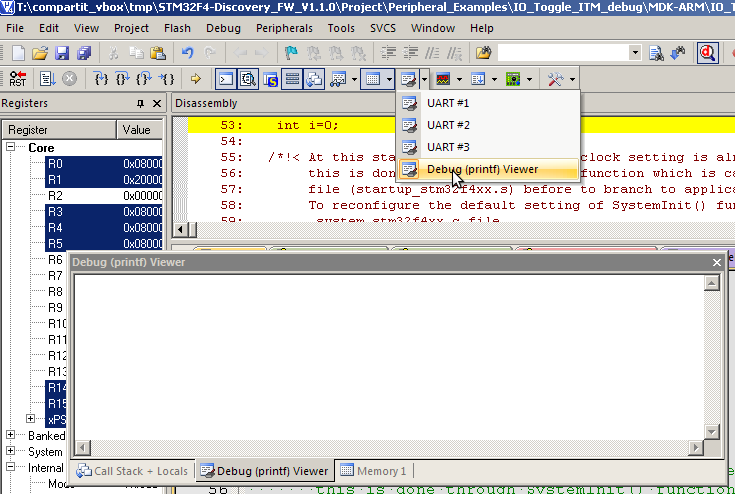
\includegraphics[scale=0.6]{keil}
                    \rule{35em}{0.5pt}
                    \caption{Keil - IDE phát triển phần mềm trên các vi xử lý họ ARM}
                    \label{fig:keil}
                \end{figure}

%================= Testing ===================================
    \section{Kiểm thử}
        Kiểm thử phần mềm nhúng có nhiều điểm giống nhau so với kiểm thử phần
        mềm ứng dụng thông thường. Tuy nhiên, có một vài điểm khác nhau giữa
        hai loại kiểm thử. Kiểm thử phần mềm nhúng thường phải truy cập đến
        những công cụ kiểm thử dựa trên phần cứng, cái thường không được sự
        dụng trong phát triển phần mềm ứng dụng.

        Kiểm thử cho điện thoại di động đương nhiên sẽ khác so với kiểm thử một
        bộ phận điều khiển của xe hơi. Mỗi công việc đều đòi hỏi định lượng
        pháp kiểm thử cho từng hệ thống riêng biệt. Không có một phương pháp
        chung nào cho tất cả các hệ thống nhúng.

        \subsection{Các giai đoạn kiểm thử}
            \begin{enumerate}
                \item Kiểm thử module
                \item Kiểm thử tích hợp
                \item Kiểm thử hệ thống (phần mềm)
                \item Kiểm thử tích hợp phần cứng - phần mềm
            \end{enumerate}
            Như vậy, so với kiểm thử thông thường thì kiểm thử phần mềm nhúng
            có thêm giai đoạn kiểm thử tích hợp phần cứng - phần mềm.

        \subsection{Một số vấn đề trong kiểm thử phần mềm nhúng}
            \begin{itemize}
                \item Kiểm thử các hệ thống thời gian thực khó bởi vì chúng
                    phản ứng với các sự kiện và dữ liệu không đồng bộ. Trên
                    thực tế gần như không thể kiểm tra một cách toàn diện các
                    trường hợp đầu vào của một hệ thống nhúng.

                \item Không thể sử dụng các phương pháp kiểm thử thông thường
                    vào một số hệ thống (vì dụ: không thể đặt breakpoint trong
                    quá trình thực thi hệ thống điều khiển máy bay khi nó đang
                    ở độ cao hàng chục km!). Nếu những hệ thống này hoạt động
                    sai, gần như không thể lặp lại chuỗi sự kiện dẫn đển lỗi để
                    tìm cách chẩn đoán.

                \item Nhiều hệ thống phụ thuộc vào trạng thái, có nghĩa là phản
                    ứng đối với một sự kiện không chỉ phụ thuộc vào sự kiện đó
                    mà còn phụ thuộc vào những gì đã xảy ra trước đó. Nói cách
                    khác, hai sự kiện giống nhau có thể dẫn đến kết quả khác
                    nhau.
            \end{itemize}

%================= Maintenance ==============================
    \section{Bảo trì}
        Về cơ bản, bảo trì phần mềm nhúng không khác với bảo trì phần mềm thông
        thường. Chúng đều có các bước chính như nhau. Tuy nhiên, do các đặc
        tính của phần mềm nhúng mà có một số yếu tố phát sinh \cite{EmbMtn}.

        \paragraph{Một số vấn đề trong bảo trì phần mềm nhúng}
            
            \begin{itemize}
                \item Các yêu cầu không ổn định:
                    Với phần mềm nhúng, các yêu cầu đuợc thêm vào và thay đổi
                    thường xuyên. Sự thay đổi thường không phải lúc nào cũng
                    có thể thông báo được đến tất cả các bên. Do đó việc bảo trì
                    trở nên rất phức tạp.

                \item Sự thay đổi về công nghệ:
                    Công nghệ phần cứng thường phát triển nhanh hơn phần mềm.

                \item Cần phải đào tạo:
                    Với một vài lĩnh vực, quá trình bảo trì phức tạp bởi rất khó để
                    hiểu được chương trình phần mềm. 

                \item Môi trường giả lập vs thiết bị thực (target):
                    Thông thường, những người phát triển phần mềm không phải ai
                    cũng có quyền tiếp xúc với thiết bị thực, việc phát triển /
                    bảo trì
                    phần mềm trở nên phụ thuộc vào môi trường giả lập.

                \item Ràng buộc về phần cứng
            \end{itemize} 
        
                
